\documentclass[11pt]{article}
\usepackage{amsmath,amsthm,amssymb,fullpage,graphicx,hyperref,listings}
\usepackage{listings,color,setspace}
\author{Andy Reagan}
\title{Math 337 Homework 13}

     \def\NN{\mathbb{N} }
     \def\ZZ{\mathbb{Z} }
     \def\QQ{\mathbb{Q} }
     \def\RR{\mathbb{R} }
     \def\CC{\mathbb{C} }
     \def\f{\frac }
     \def\b{\begin }
     \def\e{\end }
     \def\Log{\text{Log} \,}
     \def\Re{\text{Re} \, }
     \newcommand{\pdiff}[2]{\frac{\partial #1}{\partial #2}}
     \newcommand{\partialdiff}[2]{\frac{\partial #1}{\partial #2}}
     \newcommand{\pdiffsq}[2]{\frac{\partial^2 #1}{{\partial #2}^2}}
     \newcommand{\pdiffcu}[2]{\frac{\partial^3 #1}{{\partial #2}^3}}
     \newcommand{\pdiffhi}[3]{\frac{\partial^#3 #1}{{\partial #2}^#3}}
     \newcommand{\diff}[2]{\frac{{\rm d}#1}{{\rm d}#2}}
     \newcommand{\diffsq}[2]{\frac{{\rm d}^{2}#1}{{\rm d} {#2}^2}}
     \newcommand{\diffhi}[3]{\frac{{\rm d}^#3 #1}{{\rm d} {#2}^#3}}
     \newcommand{\tdiff}[2]{\mbox{d} #1/\mbox{d} #2}
     \newcommand{\tdiffsq}[2]{\mbox{d}^{2} #1/\mbox{d} {#2}^2}
     \newcommand{\tpdiff}[2]{\partial #1/\partial #2}
     \newcommand{\tpdiffsq}[2]{\partial^2 #1/\partial {#2}^2}
     \newcommand{\bvec}[1]{\vec{ {\bf #1 } }}
     \newcommand{\oh}[1]{O(h^{{#1}})}

\lstset{language=MATLAB,
basicstyle=\ttfamily\scriptsize\singlespacing,
keywordstyle=\color{black},
stringstyle=\color{black},
commentstyle=\color{black},
morecomment=[l][\color{black}]{\#},
frame=L,
xleftmargin=\parindent,
%%numbers=left,                   %% where to put the line-numbers
%%numberstyle=\scriptsize,      %% the size of the fonts that are used for the line-numbers
%%stepnumber=1,                   %% the step between two line-numbers. If it is 1 each line will be numbered
numbersep=5pt,
breaklines=true,        %% sets automatic line breaking
breakatwhitespace=false,    %% sets if automatic breaks should only happen at whitespace
escapeinside={\%*}{*)} 
}

\begin{document}
\maketitle

\begin{enumerate}

\item We start by writing the corresponding equation for (13.5) as 
\[ \f{U_m ^{n+1} - U_m ^{n} }{\kappa}  = \f{1}{2} \left [ a\f{U_{m+1} ^n -2 U_{m} ^n +U_{m-1} ^n}{h^2} + \f{1}{h^2} f(x_m ,t_n ) + a\f{U_{m+1} ^{n+1} -2 U_{m} ^{n+1} +U_{m-1} ^{n+1}}{h^2} + \f{1}{h^2} f(x_m ,t_{n+1} ) \right ] .\]
Since $f$ is known for all times $t$, we then have 
\[ \left (1-\f{ar\delta_x ^2 }{2}\right )U_m ^{n+1} = \left (1+\f{ar\delta_x ^2 }{2}\right )U_m ^{n} + \f{r}{2} \left ( f(x_m ,t_n ) + f(x_m ,t_{n+1} ) \right )  .\]
With $r = \kappa / h^2$, we write the above in vector notation 
\[ \left (1-\f{ar}{2}A\right )\bvec{U} ^{n+1} = \left (1+\f{ar}{2}A\right )\bvec{U} ^{n} + \bvec{b},\]
where the matrix $A$ is defined as in the notes (Eq 13.10) and $\bvec{b}$ is defined as
\[ \bvec{b} = \f{r}{2} \left ( \begin{array}{c} g_0 (t_n) + g_0(t_n+1) \\0\\.\\0\\ g_1 (t_n) + g_1(t_n+1) \end{array} \right ) + \f{r}{2} \left ( f( \bvec{x} ,t_{n+1} ) + f( \bvec{x} , t_n ) \right ) \].

\item For the $\theta$ family of methods, we have the discreization from Eq 13.16 as
\[ \bvec{U}^{n+1} = \bvec{U}^{n} + \kappa \left ( \left ( 1-\theta \right ) f(t_n, \bvec{U}^n ) + \theta f(t _{n+1},\bvec{U}^{n+1} ) \right ) \]
which leads to the method corresponding to Eq 13.17, which is
\[ (I-r\theta A) \bvec{U}^{n+1} = (I +r (1-\theta) A)\bvec{U}^n + \bvec{b}.\]
Following the traditional stability analysis, Eq 13.20 writes this in a form more suitable for the stability analysis (where we've dropped $\bvec{b}$ since we only need the homogeneous problem):
\[ \bvec{U}^{n+1} = (I-r\theta A) ^{-1} (I +r (1-\theta) A)\bvec{U}^n .\]
Writing this again for each node, we have
\[ (1-r\theta \partial _x ^2 ) U^{n+1} _m  =  (1 +r (1-\theta) \partial _x ^2 )U^n_m  .\]
Expanding,
\[ U^{n+1} _m-r\theta (U^{n+1} _{m+1} -2U^{n+1} _m + U^{n+1} _{m-1} )  =   U^n_{m}+r (1-\theta) (U^n_{m+1}-2U^n_{m}+U^n_{m})  .\]
Since this equation is linear, the error also obeys this difference scheme, and we write
\[ \epsilon^{n+1} _m-r\theta (\epsilon^{n+1} _{m+1} -2\epsilon^{n+1} _m + \epsilon^{n+1} _{m-1} )  =   \epsilon^n_{m}+r (1-\theta) (\epsilon^n_{m+1}-2\epsilon^n_{m}+\epsilon^n_{m})  .\]
Using the same Fourier expansions as in Chapter 12 of the notes (and my Homework 12), we have
\begin{align*} &\rho^{n+1} e^{i \beta m h}-r\theta (\rho ^{n+1} e^{i \beta (m+1) h} -2\rho ^{n+1} e^{i \beta m h}+ \rho ^{n+1} e^{i \beta (m-1) h} )\\  ~~~~~~&=   \rho ^{n} e^{i \beta m h}+r (1-\theta) (\rho ^{n} e^{i \beta (m+1) h}-2\rho ^{n} e^{i \beta m h}+\rho ^{n} e^{i \beta (m-1) h})  .\end{align*}
Cancelling the common $\rho ^n e^{i\beta mh}$ we are left with
\begin{align*} \rho -r\theta (\rho e^{i \beta h} -2\rho + \rho e^{-i \beta h} ) =   1+r (1-\theta) (e^{i \beta h}-2+ e^{-i \beta h})  .\end{align*}
Letting $z = -4r \sin ^2 \left ( \f{\beta h }{2} \right )$ we have
\begin{align*} \rho (1-\theta z) =   1+ (1-\theta) z, \end{align*}
and therefore
\begin{align*} \rho  =  \f{ 1+ (1-\theta) z} {1-\theta z}. \end{align*}
For stability we require $|\rho| < 1$ and so 
\begin{align*} &\left | \f{ 1+ (1-\theta) z} {1-\theta z} \right | < 1\\
-1 & < \f{1+ (1-\theta) z  }{1-\theta z}  < 1 \\
-1+\theta z & < 1+ (1-\theta) z < 1-\theta z \\
-2+\theta z & < z-\theta z < -\theta z \\
-2+2\theta z & < z < 0 \end{align*}
Since $z<0$ always, ($\sin^2 \in [0,1]$ and $r>0$), we now deal with:
\begin{align*} -2& < (1-2\theta) \left ( -4r \sin ^2 \left (\f{\beta h}{2} \right ) \right )\\
\f{1}{2} & > (1-2\theta) r \sin ^2 \left (\f{\beta h}{2} \right )\end{align*}
Since again $\sin ^2 \left (\f{\beta h}{2} \right ) \in [0,1]$, for the above to hold for any value of $\beta h$, we have 
\[  (1-2\theta) r < \f{1}{2}, \]
which is the same as Eq 13.27.


\item Let $\vec{v}$ be an eigenvector of $A$.
Therefore $\exists \lambda $ such that
\[A\vec{v} = \lambda \vec{v},\]
and clearly multiplying by any scalar $a$ we have
\[aA\vec{v} = a\lambda \vec{v}.\]

Also, notice that 
\[ I\vec{v} = \vec{v} = 1\cdot \vec{v} \]
where by $\cdot$ scalar mutliplication is implied.
The above equation can then, be multiplied by any scalar $b$.
Adding the two previous equations, we have
\begin{align*} aA\vec{v} bI\vec{v}  &= a\lambda \vec{v} + b\vec{v}\\ \vspace{1mm}
\Rightarrow (aA+ bI)\vec{v}  &= (a\lambda +b) \vec{v}\end{align*}
which proves that $a\lambda +b$ is an eigenvalue of $aA+ bI$ with eigenvector $\vec{v}$.

In the above derivation, replacing $a \to c, b \to d$ we have
\[ (cA+ dI)\vec{v} = (c\lambda +d) \vec{v}.\]
Taking the inverse of both sides, we have
\[ (cA+ dI)^{-1}\vec{v} = (c\lambda +d)^{-1} \vec{v},\]
which proves that $(c\lambda +d)^{-1}$ is an eigenvalue of $(cA+ dI)^{-1}$ with eigenvector $\vec{v}$.

Finally, in Eq 13.20
\[ \bvec{U} ^{n+1}  = (I - r \theta A ) ^{-1} (I + r(1-\theta ) A) \bvec{U} ^n \]
let $a = r(1-\theta) , b = 1, c = -r\theta, $  and $d=1$.
Therefore the eigenvalues of 
\[ \mathcal{M} =  (I - r \theta A ) ^{-1} (I + r(1-\theta ) A) \]
for $\lambda _j$ an eigenvalue of $A$ are
\[ (a \lambda _j + b) (c\lambda _j + d) ^{-1}  = \f{1 + r(1-\theta) \lambda _j }{1 - r\theta \lambda _j}. \]

\item I solve the IBVP using CN in the follow code:

\lstinputlisting[language=Matlab]{andy_hw13_prb04.m}

In the following two figures I present the numerical solution for each value of $\kappa$ and the error for each $\kappa$.

\begin{figure}[h!]
  \centering
    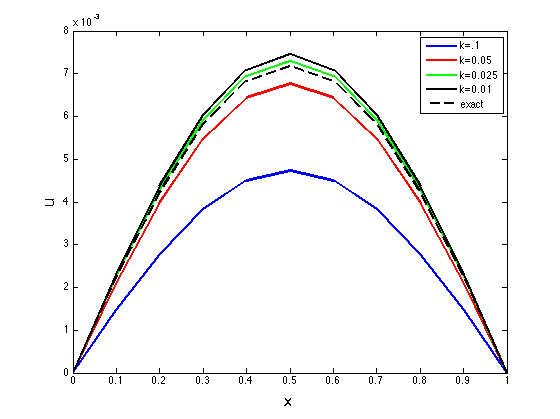
\includegraphics[width=0.45\textwidth]{andy_hw13_prb04_02.png}
  \caption{The numerical and exact solution for each $\kappa$ using the CN method on the IBVP of Problem 1, HW 12.}
\end{figure}

\begin{figure}[h!]
  \centering
    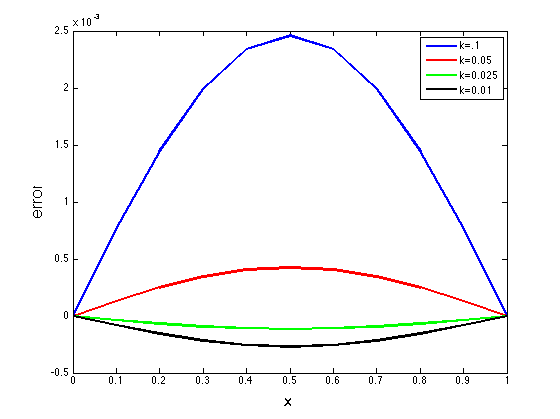
\includegraphics[width=0.45\textwidth]{andy_hw13_prb04_03.png}
  \caption{The numerical error for each $\kappa$ using the CN method on the IBVP of Problem 1, HW 12.}
\end{figure}

Questions: (i) answered in the assignment, (ii) the error changes sign because the $u_{xxxx}$ term overtakes the $u_{xxxxxx}$ term in the leading local truncation order and (iii) it increases for small $\kappa$ because the errors in $\kappa^2$ and $h^2$ do not cancel as much.

More specifically for parts (ii) and (iii), the $u_{xxxxxx}$ term has coefficient $\pi^6/12$ and the $u_{xxxx}$ has $-\pi^4/12$ so when $\kappa ^2 > h^2/pi^2$ the term in $\kappa$ dominates. Note that $1/\pi^2 \simeq .01$ so when $\kappa$ goes $0.05\to 0.025$ the error in $h$ takes over.

When $\kappa = .01$, the error in $\kappa^2$ is now smaller than it was for $\kappa = 0.025$. But, the error in $h^2$ is the same, and has been negative all along. So now that the error in $\kappa$ which was positive, is going away, the total error increases.

Finally (iv) I find the error versus $\kappa$ in a in a vector called \verb|errors|, the values of $k$ in a vector \verb|kvec| and find the exponent by fitting a line to the points in log space using least squares estimation: 

\verb| p = polyfit(log(kvec),log10(abs(errors)),1); |.

We find $p = -1.91$ indicating that the errors decrease with $\kappa$ nearly proportional to $\kappa ^2$.

\item The code which I inserted (in addition to a \verb|clear U| at line 38 so the code runs) is:

\lstinputlisting[language=Matlab,firstline=59,lastline=66]{andy_hw13_prb05.m}

I summarize my results in the follwing table:
\begin{table}[h]
  \begin{center}
    \begin{tabular}{cccc}
      \hline
$\theta$ & $p$ & $r = 1/(2h)$ & $r=1/(4h)$ \\
      \hline
      \hline
1/2 & 0  & N/A & 1.28,0.09  \\
     &  1  & N/A & N/A  \\
     &  2  & N/A & 2.1360 \\
     &  3  & N/A & 2.1002 \\
     &  4  & N/A & 2.0443 \\
1 & 0  & 1.1897 & 1.1426  \\
     &  1  & 1.1215 & 1.0773  \\
     &  2  & 1.1411 & 1.1071 \\
     &  3  & 1.1414 & 1.1076 \\
     &  4  & 1.1409 & 1.1067 \\
      \hline
    \end{tabular}
  \end{center}
\end{table}

Questions: (1) The discretization error is $O(\kappa + h^2 )$, but we observe $\gamma \approx 1$ because here $\kappa$ is large compared to $h$, as we have set $\kappa = 1/(2h)$ and $\kappa = 1/(4h)$.

(2) The solution appears jagged for $\theta = 1/2$ and $r = 1/(2h)$ all of the time. For $\theta = 1/2$ and $r = 1/(4h)$ the solution does not appear jagged, as the solution is generally stable (so we do not observe the growth of the highest frequency fourier harmonic of error near the discontinuity in the IC).

We do not observe any jaggedness for $\theta = 1$.

(3) The main difference is that for CN the solution does not become stable even for larger $p$, whereas the explicit method does become stable as the IC becomes more continuous (differentially continuous further down).

Perhaps for an IC that is known to be infinitely differentiably continuous the CN would be appropriate, but I would still stick to the explicit method for $\kappa = h/2$.

(4) In this case, I could solve the PDE with either the backwards difference ($\theta  = 1$ method with any $\kappa$, or with the explicit method with $\kappa$ such that $r$ is not near the stability threshold of $1/2$.
The solution will be more accurate for the explicit method with small $\kappa$, since the error decreases more quickly with $h$.

(5) The expression for $\rho$ was 
\begin{align*} \rho  =  \f{ 1+ (1-\theta) z} {1-\theta z}, \end{align*}
where $z = -4r \sin ^2 \left ( \beta h / 2 \right ) $.
Fixing $\beta h = \pi$ we have that $z = -4r \sin ^2 \left ( \pi / 2 \right )  = -4r $.
Therefore, 
\[ \rho _\pi = \f{1+ 4(\theta-1)r}{1+4\theta r} . \]
For $h = 0.05,$ we set $\rho$ between $[1/(2h),1/(4h)]$ and then $\kappa = h^2 r$.
Therefore we make a plot of
\[ \log \left ( \left | \f{1+ 4(\theta-1)r}{1+4\theta r} \right | ^{t_{\max} / (h^2 r) } \right ) \]
versus $r$.
I also make plots for the above, without taking the log (which I find easier to interpret).
For $\theta = 1$ we that the the harmonic $\rho _\pi$ has decreased to machine error by the time $t = 0.5$, which agrees with the stability of our solution for $\theta =1, p = 0$.

For $\theta = 1/2$, we have for $r = 1/(4h)$ that the Fourier mode represented by $\rho _\pi$ has decreased almost to 0.
This agrees with the fact that our solution was stable for this value of $r$.
But for $r = 1/(2h)$ the mode $\rho _\pi$ has yet to decay significantly, and dominates the final solution at $t = 0.5$.
If we continue to solve, this harmonic will decrease to 0, but it is still large at $t = 0.5$ and this confirms our observation that the solution at $t = 0.5$ is incorrect.

\begin{figure}[h!]
  \centering
    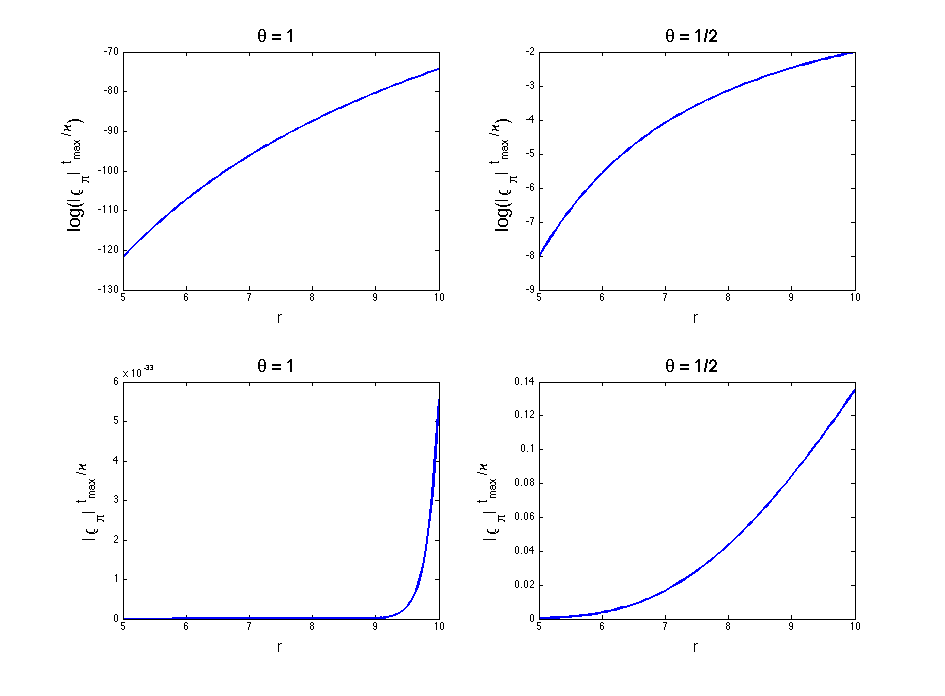
\includegraphics[width=0.8\textwidth]{andy_hw13_prb05_05.png}
  \caption{The growth factor of the Fourier mode $\rho _\pi$ at time $t = 0.5$ for the $\theta$-family of methods with $\theta = 1/2,1$.
           On the top, we take the log of the error growth, and on the bottom we plot it directly.}
\end{figure}

(6) Based on our exploration of the CN method applied to the heat equation, the choice of parameters depends on how much we know about the parabolic PDE problem we are solving, and the IC we are given.

If the IC that are given is smooth, then we need only to pick $\kappa$, $h$ such that $r<1/2$ and with $h$ such that the error is sufficiently small.

If we do not know that the IC is smooth, or even continuous, then we can still use the CN method but we need to restrict $\kappa$ such that $r$ is not near the stability threshold of $1/2$.

\clearpage
\pagebreak
\item Bonus I: First, I note that equation (13.6) is:
\[ \f{1}{\kappa} \partial _t U_{m}^{n} = \f{1}{2h^2} \left [ \partial _x ^2 U_{m}^{n} + \partial _x ^2 U_{m}^{n+1} \right ]~~~~~~~~~~~~~~~~(13.6).\]
When $\epsilon = 0$, equations (13.11) and (13.12) become
\begin{align*} U_{m}^{n+1} &= \overline{U}_{m} + \f{\kappa}{2} \overline{U}_{m,t} + \f{1}{2!} \left  ( \f{\kappa}{2} \right ) ^2 \overline{U}_{m,tt} + \f{1}{3!} \left  ( \f{\kappa}{2} \right ) ^3 \overline{U}_{m,ttt} + O (\kappa ^4) \\
U_{m}^{n} &= \overline{U}_{m} - \f{\kappa}{2} \overline{U}_{m,t} + \f{1}{2!} \left  ( \f{\kappa}{2} \right ) ^2 \overline{U}_{m,tt} - \f{1}{3!} \left  ( \f{\kappa}{2} \right ) ^3 \overline{U}_{m,ttt} + O (\kappa ^4) \end{align*}
where there is only $O(\kappa ^4)$ terms truncated because the expansion does not involve $m$.
Plugging the above two equations into the LHS of (13.6), we have 
\begin{align*} \f{1}{\kappa} \left ( U_{m} ^{n+1} - U_{m} ^{n} \right ) &= \f{1}{\kappa} \overline{U}_{m} + \f{1}{2} \overline{U}_{m,t} + \f{1}{2!} \f{\kappa}{4}  \overline{U}_{m,tt} + O (\kappa ^3)\\
&~~~~~- \left [ \f{1}{\kappa} \overline{U}_{m} - \f{1}{2} \overline{U}_{m,t} + \f{1}{2!} \f{\kappa}{4}  \overline{U}_{m,tt} + O (\kappa ^3) \right ]\\
&= \overline{U} _{m,t} \left ( \f{1}{2} + \f{1}{2} \right ) + \left ( \f{1}{3!} \f{\kappa ^2}{8} + \f{1}{3!} \f{\kappa ^2}{8} \right ) \overline{U}_{m,ttt} + O(\kappa ^2) \\
&= \overline{U} _{m,t} + O(\kappa ^2) \end{align*} 
which verifires (13.13).


Now the important observation about the truncation error of the $U_{m\pm \epsilon} ^{n+1}$ and $U_{m\pm \epsilon} ^n$: since the expansion for $\pm\epsilon$ is being added to eachother, the error terms in $\kappa^2 h$ and $h^2 \kappa$ will cancel due to the symmetry, in both the $n,n+1$ cases.
Specifically, the $\overline{U} _{m,xtt}$ (truncation error $O(\kappa ^2 h)$) cancels between different $\epsilon$ for each $n,n+1$ (since $\epsilon$ is linear and has different signs for the $U_{m\pm1}$, not appearing the $U_m$) and the $\overline{U} _{m,xxt}$ (truncation error $O(h^2 \kappa)$) cancels not within each $n,n+1$, but across them.
That is, $\kappa$ is in linear on the $\overline{U} _{m,xxt}$, so the sign is opposite between the $n,n+1$ expansions.
Here, I've only noted the cancellation of the $\kappa^2 h$ and $h^2 \kappa $ terms since we are only expanding through the second order in each, i.e. the order of truncation for each $U_{m+\epsilon} ^{n+\{0,1\}}$ will be $O(\kappa ^3 + \kappa ^2 h + h^2\kappa + h^3)$, which we can also see directly are the local truncation errors, since they are the next terms in (13.11,13.12).

Specifically, I'm using the following form of (13.11,13.12): (where $\alpha = \{ 0,-1 \}$)
\begin{align*} U_{m+\epsilon} ^{n-\alpha} &= \overline{U}_m + \left ( \f{\alpha \kappa}{2} \overline{U} _{m,t} + \epsilon h \overline{U} _{m,x} \right ) \\
&~~~~+\f{1}{2!} \left ( \left ( \f{\alpha \kappa }{2 } \right ) ^2 \overline{U} _{m,tt} + \alpha \kappa \epsilon h \overline{U} _{m,xt} + \left ( \epsilon h \right ) ^2 \overline{U} _{m,xx} \right )\\
&~~~~+O(\kappa ^3 + \kappa ^2 h + h^2\kappa + h^3) \end{align*}

Since writing out the whole expansion is not very insightful (I have done such), I will instead note directly which terms cancel, from where, when Eqs (13.11,13.12) are plugged into the RHS of Eq (13.6).
First let's talk about the $\overline{U}_m$ terms.
Since the $\delta _x ^2$ discretization has $U_{m+1} -2 U_m + U_{m-1}$ in it, and the $\overline{U}_m$ is unchanged for each, it has the coefficients $(1-2+1)=0$ and cancels in the $\delta _x ^2$, for both $n$ and $n+1$.

Next, again for each $n$ and $n+1$, the $\overline{U} _{m,tt}$ will also not change for each term in the $\delta _x ^2$.
Therefore, the coefficient will be $(1-2+1)=0$ and these terms will cancel across the $\delta$.

The term $\f{1}{2!} 2 \f{\kappa}{2} \epsilon h \overline{U} _{m,xt}$ in not contained in the middle of the $\delta_x^2$ expansion, since $\epsilon = 0$ there.
It is contained in each the $U_{m\pm 1}$ for both $n,n+1$, and there $\epsilon = \pm 1$, so they cancel with each $n,n+1$ expansion.

Finally, we deal with the $\f{1}{2!} (\epsilon h)^2 \overline{U} _{m,xx}$.
Within eacn $n,n+1$, since the $\epsilon$ is squared, the sign is the same for both the $\epsilon = \pm 1$.
Therefore, they add within each $n,n+1$.

Taking all of this together, we have proven that
\[ \f{1}{2h^2} \left [ \partial _x ^2 U_{m}^{n} + \partial _x ^2 U_{m}^{n+1} \right ] = \overline{U} _{m,xx} + O(\kappa ^2 + h ^2 ) .\]

\item Bonus II: Collecting terms in $m,n$ for the Dufort-Frankel scheme we have:
\[ (1+2r) U_{m} ^{n+1} = 2r U_{m+1} ^n + (1-2r) U_{m}^{n-1} + 2r U_{m-1} ^n. \]
Since this in linear, we replace $U$ with the error $\epsilon$ 
\[ (1+2r) \epsilon_{m} ^{n+1} = 2r \epsilon_{m+1} ^n + (1-2r) \epsilon_{m}^{n-1} + 2r \epsilon_{m-1} ^n. \]
Now we expand $\epsilon$ with a specific Fourier series, namely $\epsilon \to \rho ^n e^{i\beta m h}$:
\[ (1+2r) \rho^{n+1} e^{i\beta (m) h}= 2r \rho^{n} e^{i\beta (m+1) h}+ (1-2r) \rho^{n-1} e^{i\beta (m) h}+ 2r \rho^{n} e^{i\beta (m-1) h}. \]
Cancelling $\rho ^{n-1} e^{i\beta m h}$, we are left
\[ (1+2r) \rho^{2} = 2r \rho e^{i\beta h}+ (1-2r) + 2r \rho e^{-i\beta h}. \]
Now we turn to plotting the largest magnitude root $\rho$ for $\beta h \in [0,\pi]$ and $r \in [0,10]$.
The following code does just that:

\lstinputlisting[language=Matlab]{andy_hw13_prb07.m}

\begin{figure}[t!]
  \centering
    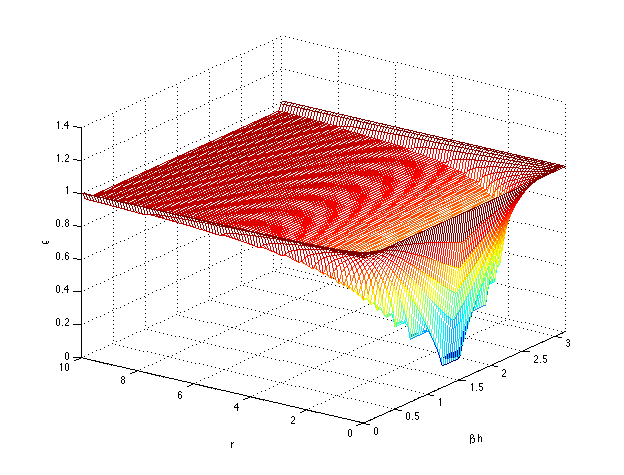
\includegraphics[width=0.45\textwidth]{andy_hw13_prb07_01.png}
  \caption{Magnitude of the largest root $\rho$ in the Von Nuemann stability analysis of the Dufort-Frankel scheme.}
\end{figure}

\end{enumerate}

\end{document}



